\section{Approach \& Background}

In order to enforce reservations while still running best effort jobs
opportunistically, our approach is use priority scheduling.

Enforcing priorities requires fewer global runqueue searches than weights do,
because they only need to happen on \textit{class boundary crossings}: on
\exit{}, when a core switches to running lower class processes after having
previously been running high class, and on \entry{}, when a core enqueues a
higher class process. 

Linux already provides priority scheduling across scheduling classes, of which
it has three that are accessible to users (in descending order of priority):
\deadlineclass{}, \rtclass{}, and \normalclass{}. Most load falls into the
\normalclass{} scheduling class, it is only within the \normalclass{} scheduling
class that the \cgroups{} weight interface is relevant.

Linux prioritizes strictly between different scheduling classes, and each class
has its own scheduling algorithm, keeps its own runqueues, and balances its own
load across cores.

\begin{figure}[t]
    \centering
    \begin{subfigure}[t]{\columnwidth}
        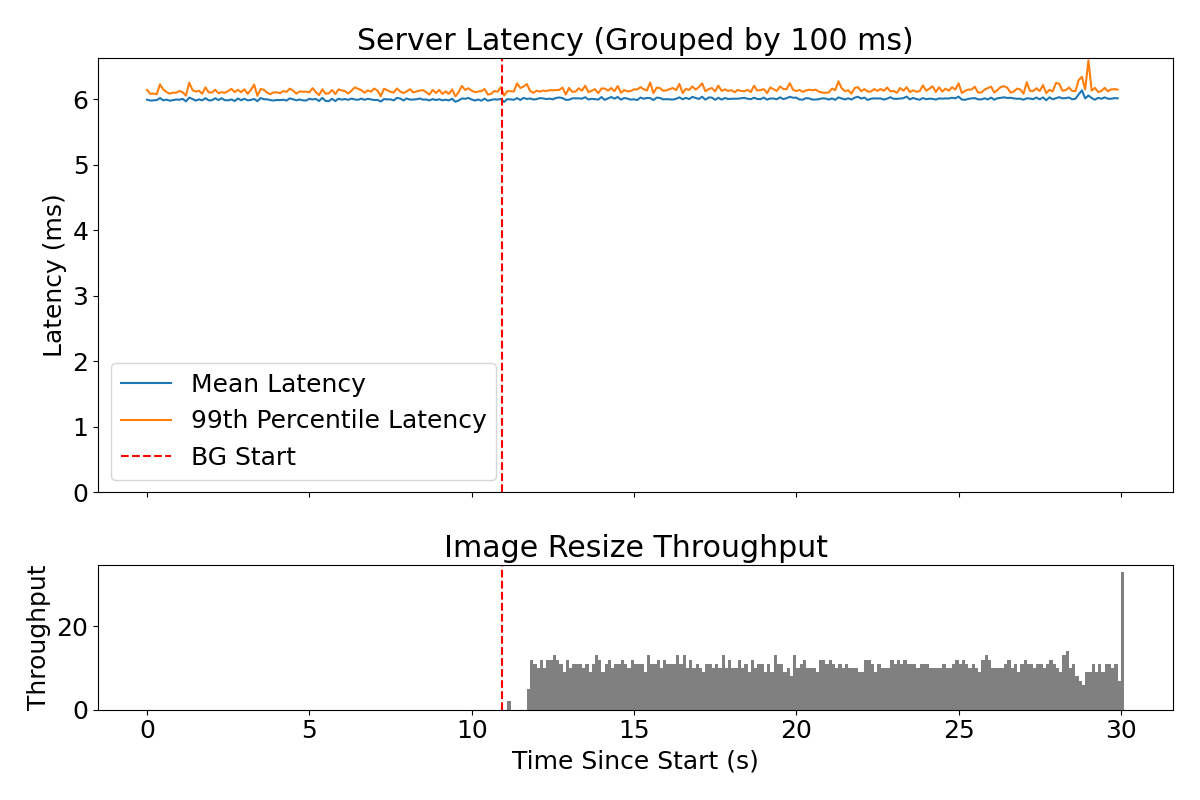
\includegraphics[width=\columnwidth]{graphs/srv-bg-rt-low.png}
        \caption{Low load (85\%)}\label{fig:srv-bg-rt-low}
        \vspace{12pt}
    \end{subfigure}
    \hspace{\fill}
    \begin{subfigure}[t]{\columnwidth}
        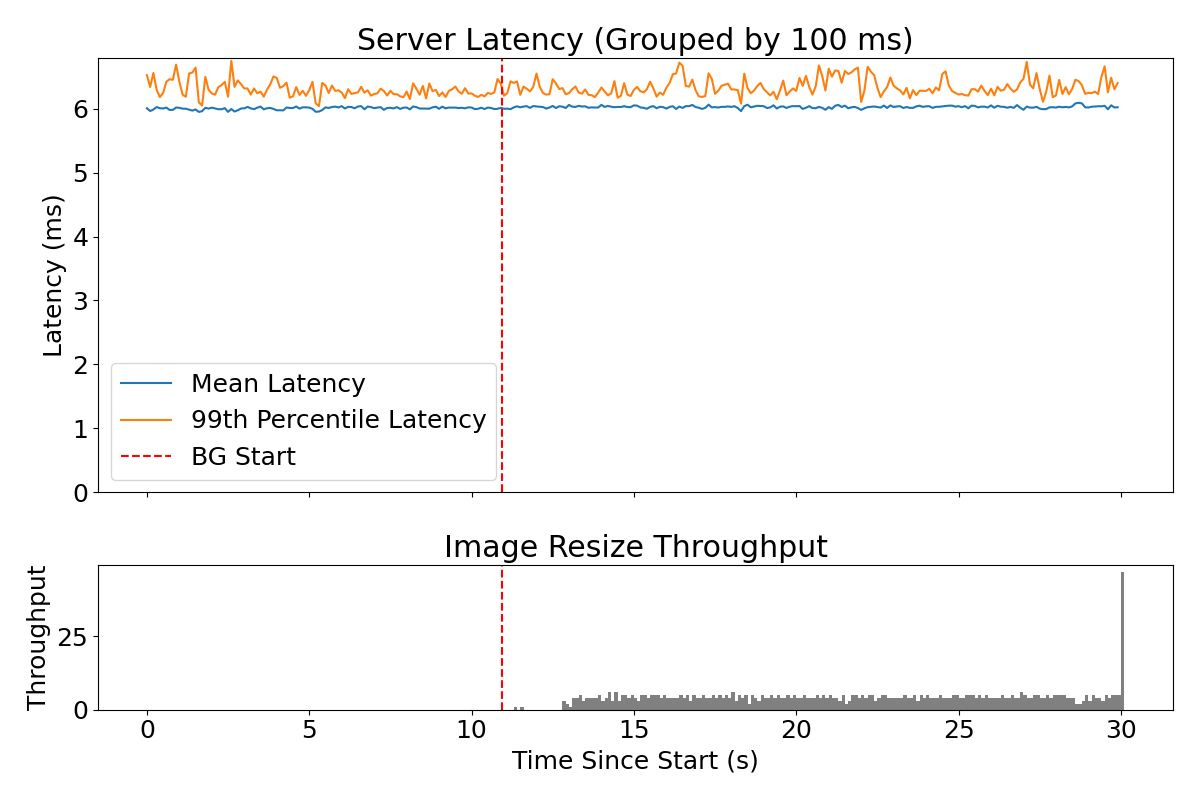
\includegraphics[width=\columnwidth]{graphs/srv-bg-rt-high.png}
        \caption{High load (95\%)}\label{fig:srv-bg-rt-high}
    \end{subfigure}
    \vspace{4pt}
    \caption{when running the server as in \rtclass{}, Linux enforces the
     server's access to its reserved cores}\label{fig:srv-bg-rt}
\end{figure}

\autoref{fig:srv-bg-rt} shows the result of running the microbenchmark with the
LC server in the \rtclass{} scheduling class. We can see that in both load
settings the tail and average latency stays stable at $\sim$6.0ms after starting
the BE workload.

However, running microservices in \rtclass{} is untenable because of
\rtclass{}'s intra-priority schedulers. Both do not support the \cgroups{}
weight interface, which although not good for scheduling LC and BE, is also used
to allocate CPU time within LC workloads; Kubernetes, for instance, allows users
to make fractional CPU requests, which are enforced using weights.